\section{Notação Visual para Atributos SAWSDL}\label{3-notacao-visual-sawsdl}

Uma especificação SAWSDL é essencialmente obtida por meio da junção dos grafos WSDL e OWL. Elementos WSDL/XSD anotados, independentemente do tipo de atributo SAWSDL (\textit{Model Reference} ou \textit{Schema Mapping}), possuem um brilho mais forte em relação aos elementos não anotados. Entretanto, quando anotados com o atributo \textit{Model Reference}, os elementos possuem uma borda grossa e vermelha. Tal característica facilita a identificação de elementos já anotados com \textit{Model Reference} em comparação a elementos não anotados. Adicionalmente, os elementos anotados com \textit{Model Reference} possuem uma aresta (linha tracejada na cor vermelha) ligando-os a uma ou mais classes OWL. A \figurename~\ref{fig:grafo-wsdl-nao-anotado-e-anotado}a ilustra elementos WSDL/XSD não anotados com \textit{Model Reference}, enquanto que a \figurename~\ref{fig:grafo-wsdl-nao-anotado-e-anotado}b ilustra elementos WSDL/XSD anotados.

\begin{figure}[h]
    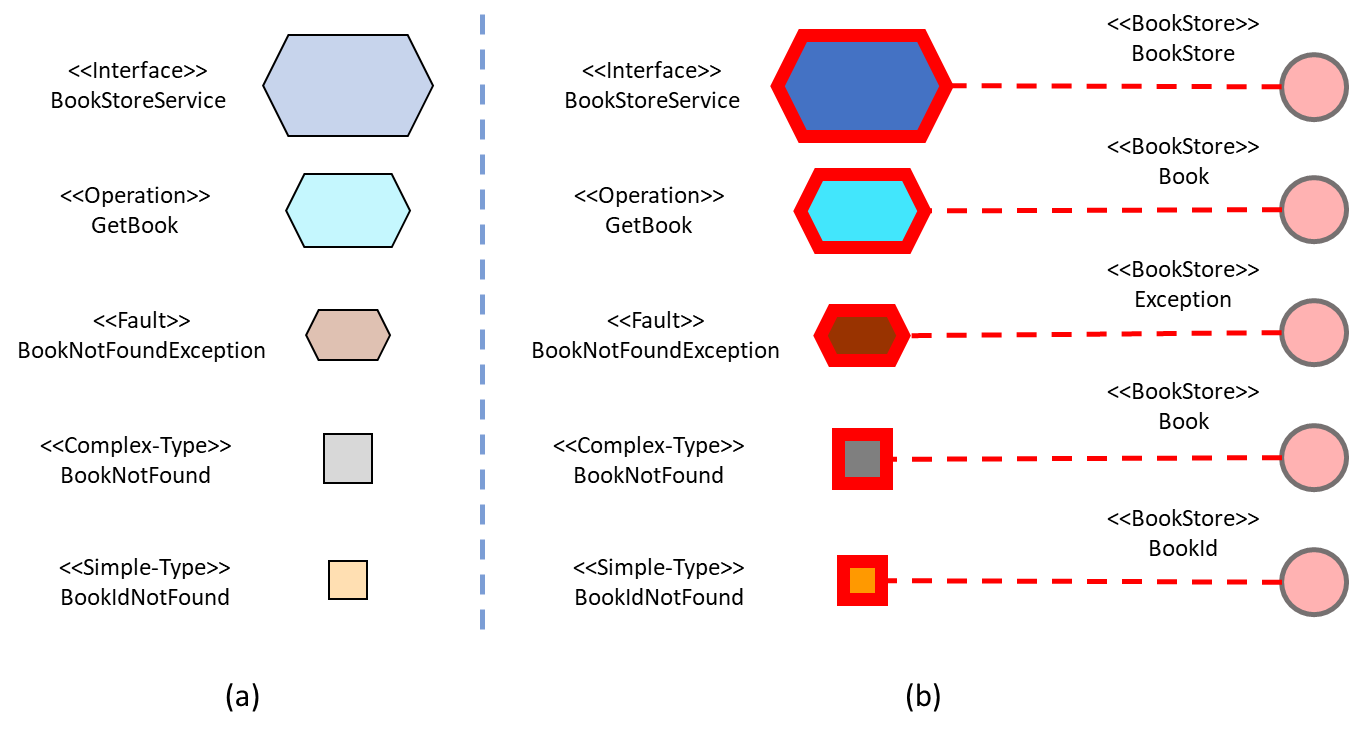
\includegraphics[scale=0.4]{3-notacao-visual-sawsdl/imagens/grafo-wsdl-nao-anotado-e-anotado.png}
    \centering
    \caption[Notação visual para elementos WSDL/XSD anotados com \textit{Model Reference}]{\textbf{Notação visual para elementos WSDL/XSD anotados com \textit{Model Reference}.} (a) Elementos WSDL/XSD não anotados. (b) Elementos WSDL/XSD anotados com classes OWL.}
    \label{fig:grafo-wsdl-nao-anotado-e-anotado}
\end{figure}

%No topo, um elemento do tipo \textit{<wsdl:interface>} é exemplificado e anotado semanticamente por meio do atributo \textit{<sawsdl:modelReference>} utilizando uma classe OWL. Abaixo de \textit{<wsdl:interface>}, um elemento do tipo \textit{<wsdl:operation>} é exemplificado e anotado semanticamente por meio do atributo \textit{<sawsdl:modelReference>} utilizando uma classe OWL. Abaixo de \textit{<wsdl:operation>}, um elemento do tipo \textit{<wsdl:input>} é exemplificado e anotado semanticamente por meio do atributo \textit{<sawsdl:modelReference>} utilizando uma classe OWL. Abaixo de \textit{<wsdl:input>}, um elemento do tipo \textit{<wsdl:output>} é exemplificado e anotado semanticamente por meio do atributo \textit{<sawsdl:modelReference>} utilizando uma classe OWL. Abaixo de \textit{<wsdl:output>}, um elemento do tipo \textit{<wsdl:fault>} é exemplificado e anotado semanticamente por meio do atributo \textit{<sawsdl:modelReference>} utilizando uma classe OWL. Abaixo de \textit{<wsdl:fault>}, um elemento do tipo \textit{<xs:complexType>} é exemplificado e anotado semanticamente por meio do atributo \textit{<sawsdl:modelReference>} utilizando uma classe OWL. Por fim, abaixo de \textit{<xs:complexType>}, um elemento do tipo \textit{<xs:simpleType>} é exemplificado e anotado semanticamente por meio do atributo \textit{<sawsdl:modelReference>} utilizando uma classe OWL.

Quando os elementos WSDL/XSD são anotados com o atributo \textit{Schema Mapping}, estes elementos possuem uma borda dupla. Tal característica facilita a identificação de elementos já anotados com \textit{Schema Mapping} em comparação a elementos não anotados.

A \figurename~\ref{fig:grafo-wsdl-anotado-model-reference-e-schema-mapping} ilustra um grafo WSDL com diferentes anotações SAWSDL. O tipo complexo \texttt{Book} e a operação \texttt{GetBook} ilustram elementos WSDL anotados apenas com o atributo \textit{Model Reference}. O tipo complexo \texttt{BookNotFound} e o tipo simples \texttt{BookId} ilustram elementos WSDL anotados apenas com um atributo \textit{Schema Mapping}. Finalmente, o tipo simples \texttt{BookName} ilustra um elemento WSDL anotado tanto com o atributo \textit{Model Reference} quanto com um atributo \textit{Schema Mapping}. Este elemento possui uma borda dupla na cor vermelha.

\begin{figure}[h]
    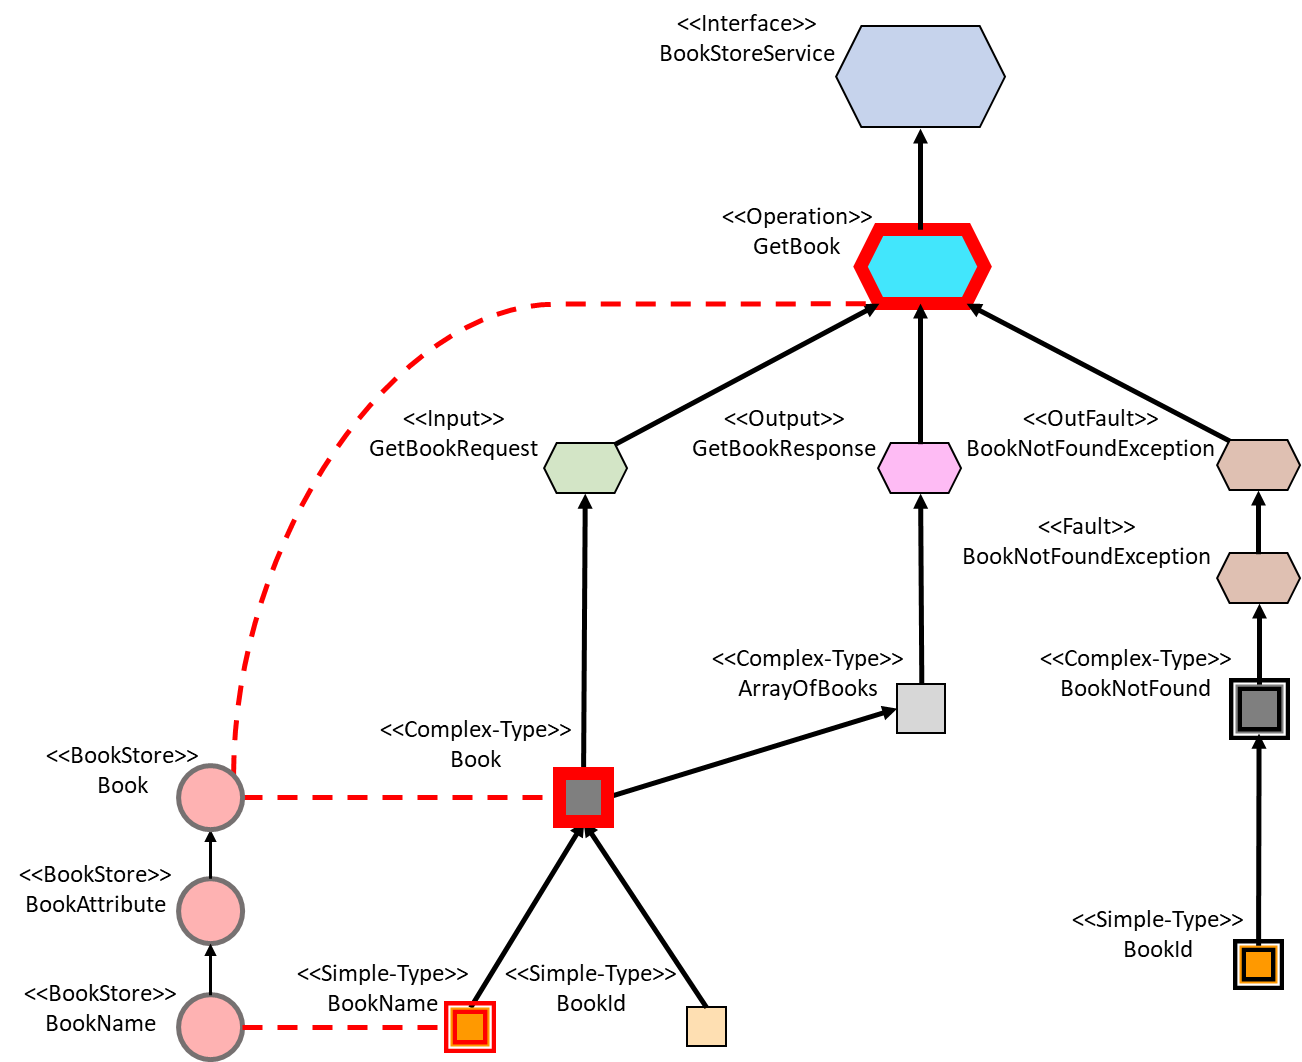
\includegraphics[scale=0.4]{3-notacao-visual-sawsdl/imagens/grafo-wsdl-anotado-model-reference-e-schema-mapping.png}
    \centering
    \caption[Exemplo de grafo WSDL com anotações utilizando tanto \textit{Model Reference} quanto \textit{Schema Mapping}]{\textbf{Exemplo de grafo WSDL com anotações utilizando tanto \textit{Model Reference} quanto \textit{Schema Mapping}.}}
    \label{fig:grafo-wsdl-anotado-model-reference-e-schema-mapping}
\end{figure}